% !TEX encoding = UTF-8 Unicode
%!TEX TS-program = xelatex

\documentclass[12pt]{extarticle}
% extarticle is like article but can handle 8pt, 9pt, 10pt, 11pt, 12pt, 14pt, 17pt, and 20pt text

\def \ititle {Origins of Mind}
 
\def \isubtitle {Lecture 08}
 
\def \iauthor {Stephen A. Butterfill}
\def \iemail{s.butterfill@warwick.ac.uk}
\date{}

%for strikethrough
\usepackage[normalem]{ulem}

\usepackage{pdfpages}


\input{$HOME/Documents/submissions/preamble_steve_handout}

%logic symbol \leftmodels
\usepackage{MnSymbol}

%\bibpunct{}{}{,}{s}{}{,}  %use superscript TICS style bib
%remove hanging indent for TICS style bib
%TODO doesnt work
\setlength{\bibhang}{0em}
%\setlength{\bibsep}{0.5em}


%itemize bullet should be dash
\renewcommand{\labelitemi}{$-$}

\begin{document}

%\raggedcolumns

\begin{multicols*}{3}

\setlength\footnotesep{1em}


\bibliographystyle{newapa} %apalike

%\maketitle
%\tableofcontents




%--------------- 
%--- start paste


\def \ititle {Logic I}
 
\def \isubtitle {Lecture 13}
 
\begin{center}
 
{\Large
 
\textbf{\ititle}: \isubtitle
 
}
 
 
 
\iemail %
 
\end{center}
 
Readings refer to sections of the course textbook, \emph{Language, Proof and Logic}.
 
 
 
\section{There Is a Store for Everything}
 
\emph{Reading:} §11.2, §11.3
 
There is a store for everything:
 
\hspace{3mm}	∃y∀x StoreFor(y,x)
 
\hspace{3mm} ∀y∃x StoreFor(x,y)
 
Other sentences to translate:
 
\hspace{3mm} Wikipedia has an article about everything
 
\hspace{3mm} Everyone hurts someone they love
 
\hspace{3mm} Someone hurts everyone she loves
 
 
 
\section{How Big Is a Truth-Table?}
 
How many truth-functions can be constructed using 2 sentence letters?
 
\begin{center}
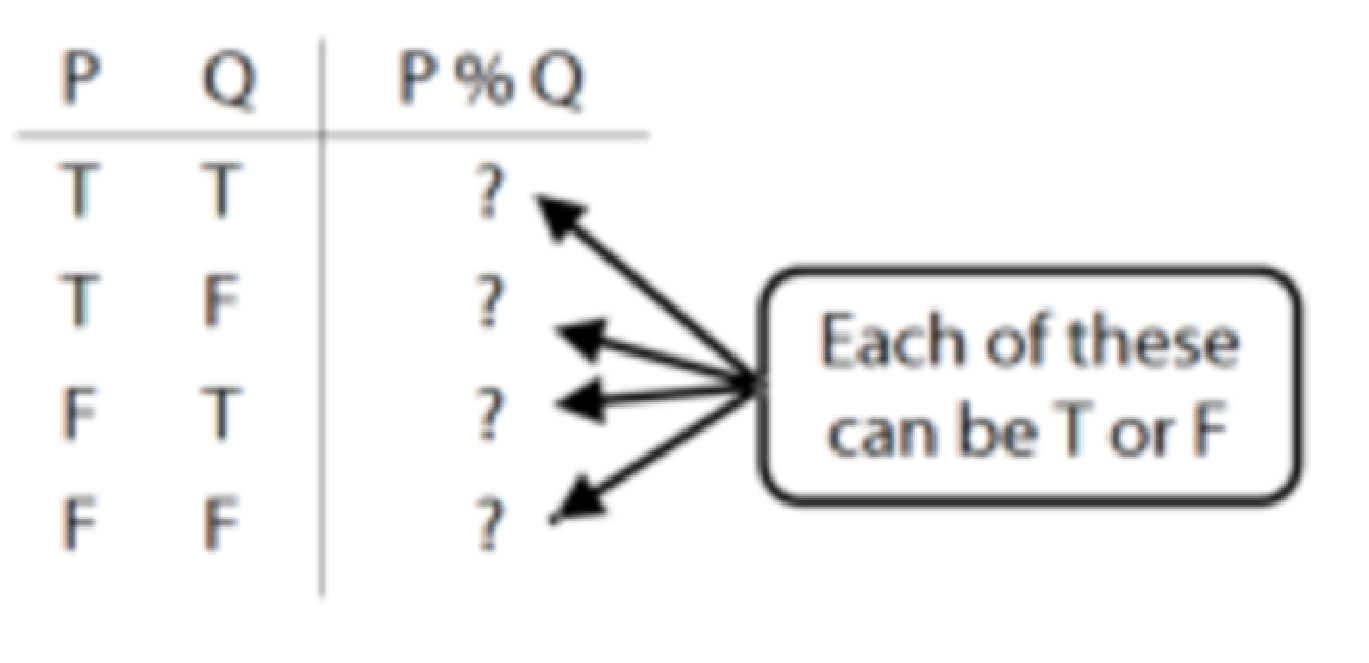
\includegraphics[scale=0.3]{img/unit_430_fig1.pdf}
\end{center}
 
 
\section{Truth-functional completeness}
 
\emph{Reading:} §7.4
 
‘A set of truth-functors is said to be \emph{expressively adequate} (or sometimes \emph{functionally complete}) iff, for every truth-function whatever, there is a formula containing only those truth-functors which express that truth-function, i.e. which has as its truth-table the truth-table specifying that function.’ (Bostock, \emph{Intermediate Logic} p. 45)
 
Illustration of the proof that $\{$¬, ∧, ∨$\}$ is truth-functionally complete:
 
\begin{center}
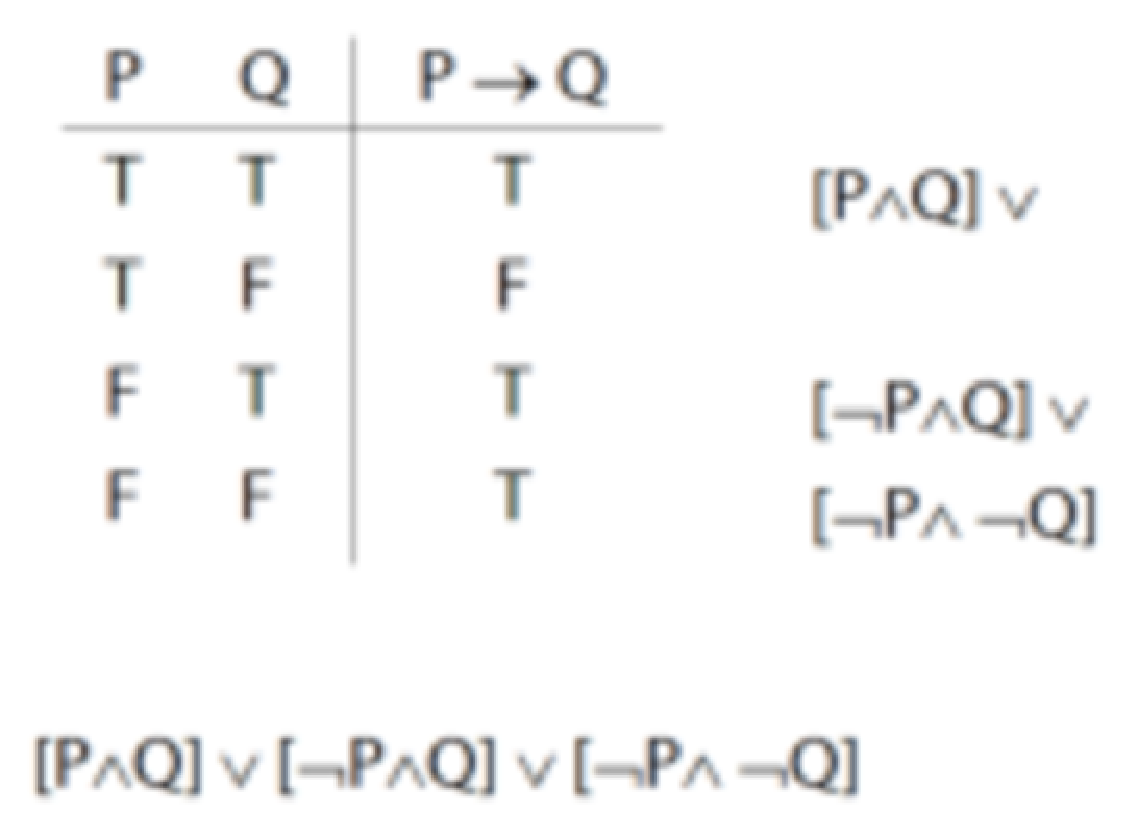
\includegraphics[scale=0.3]{img/unit_430_fig2.pdf}
\end{center}
\emph{Exercise} assuming $\{$¬,∨,∧$\}$ is truth-functionally complete, show that $\{$¬,∨$\}$ is.
 
\vfill
\begin{minipage}{\columnwidth}
\section{Exercises}
These exercises will be discussed in seminars the week after this lecture.
The numbers below refer to the numbered exercises in the course textbook, e.g.\ `1.1' refers to exercise 1.1. on page 39 of the second edition of \emph{Language, Proof and Logic}. Exercises marked `*' are optional.
 
\begin{quote}
10.24–7, *10.28–9
 
11.3
 
11.4, 11.8, 11.9
 
7.25, 7.26, *7.28, 7.29
 
\end{quote}
\end{minipage}

%--- end paste
%--------------- 
 


\end{multicols*}

\end{document}